\newpage
\chapter*{Introduction}
\addcontentsline{toc}{chapter}{Introduction}
%This is typically an outline description detailing the background to the problem.

%
\begin{figure}[ht]
	\centering
	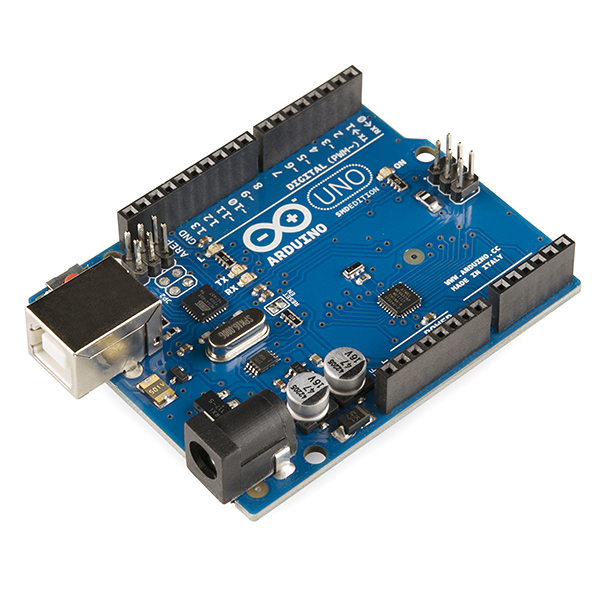
\includegraphics[width=8cm]{images/01}
	\caption{Arduino Uno R3 \citep{wikipedia-13}}
	\label{fig:arduino_uno_r3}
\end{figure}
%

Example of the glossary tag being used \gls{Arduino}.

%
\begin{table}
	\centering
	\begin{tabular}{p{4cm} l}
		\toprule
		Column 1 & Column 2\\ \midrule
		x & 1 \\
		y & 2 \\
		z & 3 \\
		\bottomrule
	\end{tabular}
	\caption{Table Caption}
	\label{tab:table_label}
\end{table}
%